\chapter{Quantum correlations in the weakly-interacting Bose gas}

\label{sec:chapter_1}

\NOTE{TOUT CECI EST MAL ECRIT, A FAIRE EN FONCTION DES ARGUMENTS DE L'INTRO}

One of the key and on-going challenges of quantum mechanics is to understand macroscopic systems containing a large number of particles $N$, commonly referred as many-body physics. Trying to consider all the possible degrees of freedom of each individual particle and interactions effects would result in an incredibly complex problem impossible to solve theoretically. Studying such systems thus require to use approximations ...

Physicists were able to describe a gas of a large number of bosonic particles with increasing complexity throughout history. The first step was the development of statistical physics, aiming to build a bridge between the microscopic properties of individual atoms or molecules and macroscopic properties of bulk materials described by thermodynamics. This approach culminated in the theory of the ideal Bose gas, ideal meaning here that all particles are non-interacting. This theory found great success with the notable prediction of a new state of matter, the Bose-Einstein condensate. 

The next step was then to increase the complexity of the problem by adding interactions between the particles. ...

While also greatly successful, the mean-field approach neglects by essence interaction phenomena between individual particles. To characterize such effects, we thus need to go beyond the mean-field approximation. ...




\section{Correlation functions in Optics}

\subsection{First order correlation function of light}

Let us begin our journey with correlation functions with the simple example of the classical description of light. Correlation functions of light were developed in strong connection with the notion of \textbf{coherence} characterizing the possibility for waves to interfere. A light field is said to be coherent when there is a fixed phase relationship for the electric field at different positions (spatial coherence) and different times (time coherence). 


\begin{figure}
    \centering
    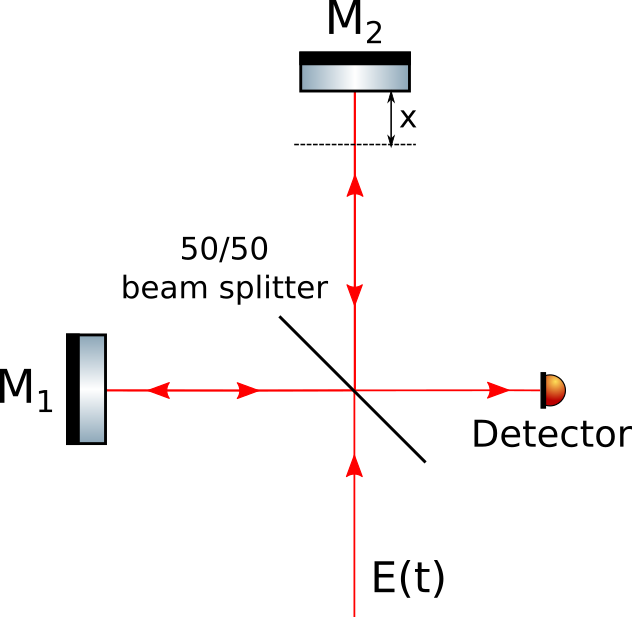
\includegraphics[width=0.55\textwidth]{Fig/Chapter1/michelson.png}
    \caption{Principle of the Michelson interferometer.}
    \label{fig:michelson}
\end{figure}


To illustrate where correlation functions come from, let us begin by taking a look at time coherence in the emblematic Michelson interferometer (see Fig.-\ref{fig:michelson}). For simplicity sake, we will not yet discuss spatial coherence effects and will thus consider a punctual source producing a complex light field $E(t)$ that we send into the interferometer. The intensity measured by the detector writes:

\begin{equation}
    I=\mean{\abs{E(t)+E(t-\tau)}^2}
    \label{eq:i_michelson}
\end{equation}

\noindent where $\mean{...}$ denotes the time average made by the detector and $\tau=\frac{2x}{c}$ the delay between the two interfering waves induced by the optical path difference between the two arms of the interferometer. Developing equation \ref{eq:i_michelson} we get:

\begin{equation}
    I=\mean{\abs{E(t)}^2} + \mean{\abs{E(t-\tau)}^2} + 2 {\rm{Re}} \mean{E(t) E^*(t-\tau)}
    \label{eq:def_g1}
\end{equation}

For simplicity sake, let us assume that the source is stationary to write $\mean{\abs{E(t)}^2} = \mean{\abs{E(t-\tau)}^2} = I_0$, we then obtain :

\begin{equation}
    I= 2 I_0 (1 + {\rm{Re}} (g^{(1)} (\tau))) \ , \ g^{(1)} (\tau) = \frac{ \mean{E(t) E^*(t-\tau)}}{\mean{\abs{E}^2}}
\end{equation}

\noindent We have introduced the normalized \textbf{first-order correlation function} $g^{(1)}$ that characterizes the interference term. If $E(t)$ and $E(t-\tau)$ are independent random variables and thus uncorrelated, $\mean{E(t) E^*(t-\tau)} = \mean{E(t)} \mean{ E^*(t-\tau)}=0$ and interference cannot be observed. On the other hand, if there is a \textbf{correlation} between these two quantities, an interference phenomenon can be observed. 

To illustrate what kind of information are contained in this first-order correlation function, let us compute it for the simple case of a monochromatic light source of frequency $\omega_0$. The light field writes:

\begin{equation}
    E(t)=E_0 e^{i \omega_0 t}
\end{equation}

\noindent From this, we calculate the first-order correlation function:

\begin{equation}
    g^{(1)} (\tau) = \frac{|E_0|^2 \mean{e^{i\omega_0 t} e^{i \omega_0 (t-\tau)}}}{|E_0|^2} = e^{i \omega_0 \tau}
\end{equation}

\noindent The detected intensity is thus a perfect sinusoidal function of $\tau$ that is scanned by changing the position of the second mirror and thus the value of $x$:

\begin{equation}
I(x)= 2 I_0 (1+\cos(\omega_0 \frac{2x}{c}))
\end{equation}

Measuring the intensity pattern as a function of $x$ thus gives a measurement of $\omega_0$. What happens if we make things slightly more complex with a light source with two monochromatic components $\omega_1$ and $\omega_2$? The new light field writes:

\begin{equation}
    E(t)= E_1 e^{i \omega_1 t} + E_2 e^{i \omega_2 t}
\end{equation}

\noindent Let us compute the numerator of the first-order correlation function:

\begin{equation}
       \mean{E(t) E^*(t-\tau)} & = \mean{|E_1|^2 e^{i \omega_1 \tau} + |E_2|^2 e^{i \omega_2 \tau} + E_1 E_2^* e^{i \omega_2 \tau} e^{i (\omega_1 - \omega_2)t} + E_2 E_1^* e^{i \omega_1 \tau} e^{i (\omega_2 - \omega_1)t}}  
\end{equation}

\noindent In most practical situations, the detector time average is large compared to $1/(\omega_1 - \omega_2)$, the two last terms thus get averaged out. If we consider the simple case where $|E_1|^2=|E_2|^2$, the normalized first-order correlation function writes:

\begin{equation}
    g^{(1)} (\tau) = \frac{1}{2} (e^{i \omega_1 \tau} + e^{i \omega_2 \tau})
\end{equation}

\noindent We simply get the sum of the contribution of the two frequencies. The intensity pattern as a function of $x$ is thus the sum of two cosine functions with different frequencies. Using trigonometric identities, we find that the intensity pattern consists of a ``fast'' oscillation of frequency $\omega_0=(\omega_1 + \omega_2)/2$, modulated by a ``slow'' oscillation of frequency $\Delta \omega = |\omega_1 - \omega_2|$, reducing the visibility of the interference pattern (see Fig.-\ref{fig:michelson_two_lambda}).

\begin{figure}
    \centering
    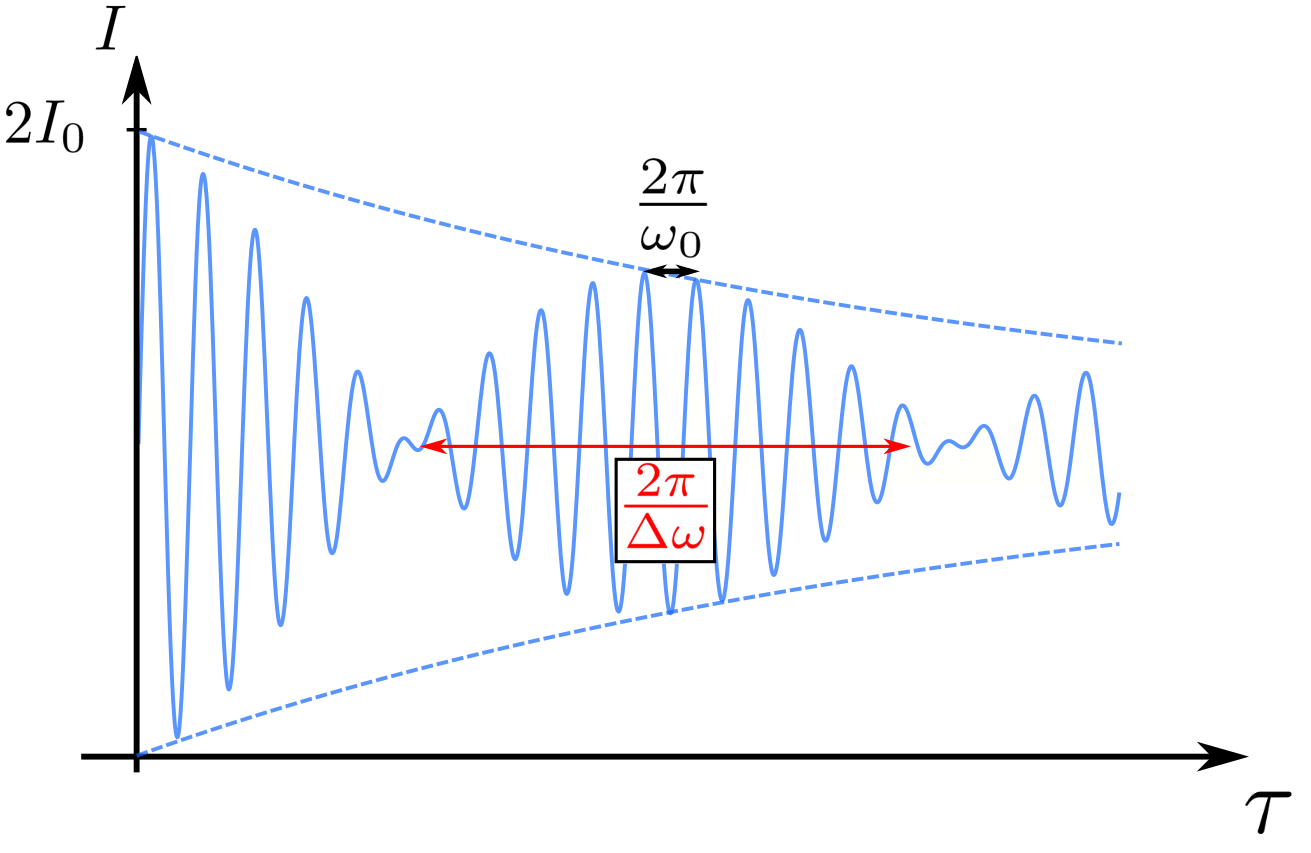
\includegraphics[width=0.78\textwidth]{Fig/Chapter1/michelson_two_lambda.png}
    \caption{Intensity pattern for a light source with two monochromatic component of frequencies $\omega_1$ and $\omega_2$. The fast oscillation of frequency $\omega_0=(\omega_1+\omega_2)/2$ is modulated by a slow oscillation of frequency $\Delta \omega = |\omega_1 - \omega_2|$.}
    \label{fig:michelson_two_lambda}
\end{figure}

Through this very simple example, we understand that the observed interference pattern strongly depends on the spectrum of the source. For a source with an arbitrary spectrum $S(\omega)$, the overall intensity pattern results of the sum of the contribution of each spectral component:

\begin{equation}
    I=\int_{-\infty}^{\infty} 2 S(\omega)[1+\cos (\omega \tau)] \mathrm{d} \omega
\end{equation}

\noindent Writing $\int_{-\infty}^{\infty} S(\omega) \mathrm{d} \omega=I_{0}$ and $s(\omega)=S(\omega) / I_{0}$, we obtain

\begin{equation}
    I=2 I_{0}\left[1+\int_{-\infty}^{\infty} s(\omega) \cos (\omega \tau) \mathrm{d} \omega\right]
\end{equation}

\noindent Since $s(\omega)$ is real, we can rewrite:

\begin{equation}
    I=2 I_{0}\left[1+\mathrm{Re} \left(\int_{-\infty}^{\infty} s(\omega) \cos (\omega \tau) \mathrm{d} \omega\right)\right]
\end{equation}

\noindent From which we get, using equation \ref{eq:def_g1}:

\begin{equation}
    g^{(1)}(\tau)=\int_{-\infty}^{\infty} s(\omega) \mathrm{e}^{\mathrm{i} \omega \tau} \mathrm{d} \omega
\end{equation}

\noindent where we recognize the definition of the Fourier transform. This is the \textbf{Wiener-Khintchine} theorem. We have thus seen that the first-order correlation function, measurable with an interferometric measurement, contains information about the spectrum of the light source. 



% Note that this is only one example in the ensemble of the many possible applications of the study of first-order correlation. We can also quote for instance the characterization of the spatial coherence of a non punctual source with the famous Young's slits experiment. 

In this introductory paragraph, we have seen a concrete and evocative example of how correlation functions can be used to obtain meaningful information about a given system, here a light source, with the simplest correlation function there is, correlating two values of the light field. At this point, the link with our initial goal, {\it i.e.} characterizing quantum many-body interacting systems, does not seem so clear. As we mentioned earlier, interactions induce correlations between several particles for which we will need higher order correlation functions. Let us now take the next step in this direction and look at \textbf{second-order correlation functions}. For the moment, we will keep things simple and work in the context of Optics, and thus with non-interacting particles, for which this formalism was historically developed and that provides well-known, easy to understand examples.

% The same reasoning can be conducted for the spatial coherence for instance with the non less famous Young double slit experiment. 

% We will not detail here all the intricacies of the study of first-order correlation functions for different light sources. The main point to remember is that the first order correlation function is a natural way to characterize the coherence properties of a light source and thus contains a lot of meaningful information.


\subsection{Second order correlation function of light: The Hanbury Brown and Twiss effect}

\begin{figure}
    \centering
    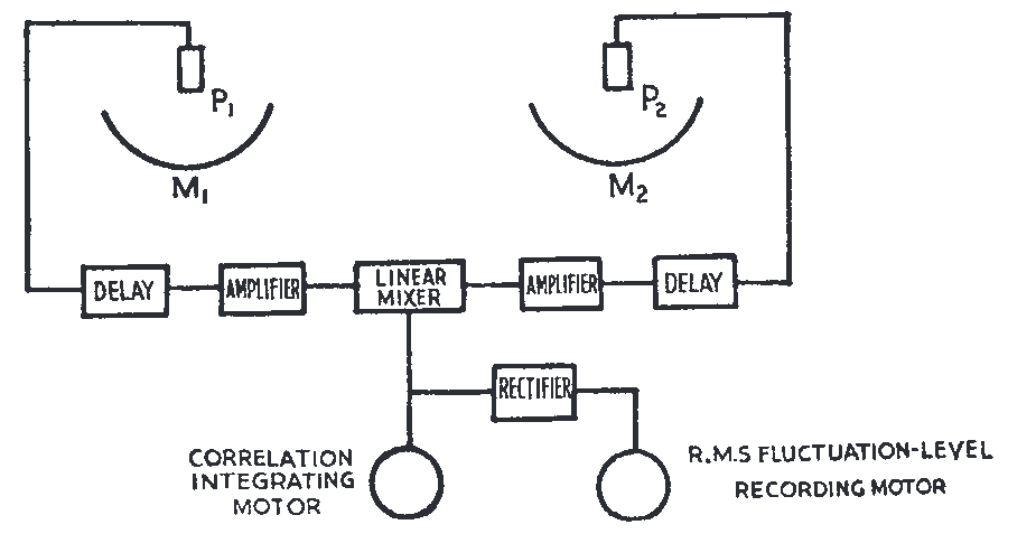
\includegraphics[width=0.7\textwidth]{Fig/Chapter1/HBT_apparatus.png}
    \caption{Diagram of the historical Hanbury Brown and Twiss apparatus, taken from \cite{brown1956test}. The novelty of this apparatus was to use two detectors, $P_1$ and $P_2$, to measure the second-order correlation function.}
    \label{fig:HBT_apparatus}
\end{figure}

\label{sec:hbt_classical}

In their really famous 1955 article \cite{brown1954lxxiv}, Hanbury Brown and Twiss proposed a new scheme relying on the measurement of cross-correlations between the intensities measured by two independent photodetectors (see Fig-\ref{fig:HBT_apparatus}), \ie a measurement of the second-order correlation function, as a mean to improve the resolution of the Michelson interferometer for measuring the size of the stars. To understand how it works, we will follow the complementary approach to the one developed in the last paragraph and look at the spatial properties of the light source. 

We consider an incoherent, non-punctual, monochromatic (wavelength $\lambda$) light source and write $S$ the surface of the source. We model it as an ensemble of elementary, punctual and independent emitters and note their spatial location $\bm{s}$. The amplitude at a point $\bm{r}$ in an observation plane situated at distance $L$, far-away from the source so that we are in the Fraunhofer regime $L \gg \lambda, r,s$, writes (see Fig-.\ref{fig:source_and_plane}):

\begin{equation}
    A(\bm{r}) \propto \int_{S} a(\bm{s}) e^{\frac{i \pi}{\lambda L}|\bm{r}-\bm{s}|^{2}} d \bm{s}
    \label{eq:amp_HBT}
\end{equation}

\begin{figure}
    \centering
    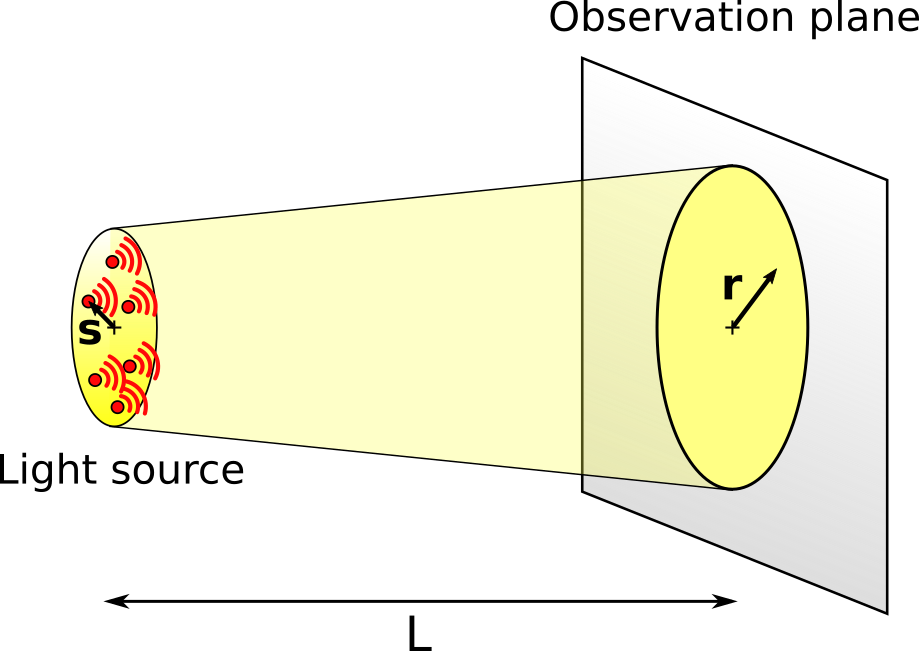
\includegraphics[width=0.7\textwidth]{Fig/Chapter1/source_and_plane.png}
    \caption{Schematic of an extended light source. The small red dots represent the different incoherent elementary emitters of the source.}
    \label{fig:source_and_plane}
\end{figure}

The second-order correlation function correlates the values of the intensity of the light field at two different points of space $\bm{r}_1$ and $\bm{r}_2$. In terms of field amplitude, it corresponds to the four-term correlator:

\begin{equation}
    G^{(2)} (\bm{r}_1,\bm{r}_2) = \mean{A^*(\bm{r}_1) A(\bm{r}_1) A^*(\bm{r}_2) A(\bm{r}_2)}
\end{equation}

\noindent All the elementary emitters are incoherent and thus each have a random phase value, determined by an uniform probability law defined on the interval $[0,2\pi]$. They thus form an ensemble of \textbf{independent} random variables with the \textbf{same statistics}. We can therefore apply the Central Limit Theorem to find that the variable $A$ follows Gaussian statistics \cite{goodman2007speckle}. This allows us to simplify the four-term correlator into:

\begin{equation}
     G^{(2)} (\bm{r}_1,\bm{r}_2) = \mean{I(\bm{r}_1)} \mean{I(\bm{r}_2)} + \mean{A^*(\bm{r}_1) A(\bm{r}_2)} \mean{A(\bm{r}_1) A^*(\bm{r}_2)}
\end{equation}

\noindent We recognize in the second term the spatial counterpart of the temporal first-order correlation function discussed in the previous paragraph. Using equation \ref{eq:amp_HBT}, we obtain:

\begin{equation}
    G^{(1)}\left(\bm{r}_{1}, \bm{r}_{2}\right)=\left\langle A^*(\bm{r}_1) A(\bm{r}_2)\right\rangle \propto \iint_{S}\left\langle a^{*}(\bm{s}_1) a(\bm{s}_2)\right\rangle e^{-\frac{i \pi}{\lambda L}\left(\left|\bm{r}_{1}-\bm{s}_1\right|^{2}-\left|\bm{r}_{2}-\bm{s}_2\right|^{2}\right)} \mathrm{d} \bm{s}_1 \mathrm{d} \bm{s}_2
\end{equation}

\noindent Since the source is incoherent, we simplify $\left\langle a^{*}(\bm{s}_1) a(\bm{s}_2)\right\rangle = I(\bm{s}_1) \delta_{\bm{s}_1,\bm{s}_2}$, giving

\begin{equation}
    G^{(1)}\left(\bm{r}_{1}, \bm{r}_{2}\right) \propto \iint_{S} I(\bm{s}_1) e^{-\frac{2 i \pi}{\lambda L}\left(\bm{r}_{1}-\bm{r}_{2}\right) \bm{s}_1} \mathrm{d} \bm{s}_1 d \bm{s}_2
\end{equation}

\noindent In analogy with what we showed in the last paragraph for the temporal coherence, the first-order spatial correlation function is the Fourier transform of the spatial intensity profile. This is known as the \textbf{Van Cittert-Zernike} theorem. For a homogeneous intensity distribution of the source, the first-order correlation function decays on a length scale called the \textbf{correlation length} $l_c$ proportional to the inverse of the source size $L_{\mathrm{source}}$, $l_c \sim \lambda L / L_{\mathrm{source}}$.

In a nutshell, the second-order normalized correlation function has the simple expression:

\begin{equation}
    \gtwo (\bm{r}_1,\bm{r}_2) = \frac{\mean{I(\bm{r}_1)} \mean{I(\bm{r}_2)} + \mean{A^*(\bm{r}_1) A(\bm{r}_2)} \mean{A(\bm{r}_1) A^*(\bm{r}_2)}}{\mean{I(\bm{r}_1)}\mean{I(\bm{r}_2)}} = 1 + |g^{(1)}(\bm{r}_1,\bm{r}_2)|^2
\end{equation}

\noindent Depending on the positions of the detectors $\bm{r}_1$ and $\bm{r}_2$ we have:

\begin{itemize}
    \item $\gtwo (\bm{r}_1,\bm{r}_2)=2$ for $\bm{r}_1=\bm{r}_2$
    \item $1 \leq \gtwo (\bm{r}_1,\bm{r}_2) \leq 2$ for $|\bm{r}_1-\bm{r}_2| \lesssim l_{c}$
    \item $\gtwo (\bm{r}_1,\bm{r}_2)=1$ for $|\bm{r}_1-\bm{r}_2| \gg l_{c}$
\end{itemize}

\noindent The size of the source can thus be obtained by progressively increasing the distance between the two detectors and measuring the length scale on which the second order correlation function decreases. This was done successfully by Hanbury Brown and Twiss \cite{brown1956test} to measure the size of Sirius in 1956.

If we take a deeper look at what happens for $\bm{r}_1=\bm{r}_2$, we see that a peculiar phenomenon occurs. The normalized second-order correlation function can be interpreted as the probability to detect simultaneously two photons on the detector located at $\bm{r}_1$ and $\bm{r}_2$, normalized by the probability to detect them independently. Therefore, since $\gtwo (\bm{r}_1,\bm{r}_2)=2$ for $\bm{r}_1=\bm{r}_2$, the probability to detect two photons at the same position is twice as high as it is to detect them independently! This effect has been named the Hanbury Brown and Twiss effect or \textbf{bosonic bunching}. While this effect bears a fully classical explanation for non quantized light fields, its quantum interpretation puzzled the physicists of the time. It was only after a few years that an explanation was suggested by Fano in 1961 \cite{fano1961quantum}. Considering a pair of source points A and B and two detectors 1 and 2, Fig-.\ref{fig:HBT_scheme} illustrates the two possibilities for a joint detection of two photons on the couple of detectors. For indistinguishable photons, the paths amplitudes interfere constructively resulting in a joint detection probability higher than for independent events. While the interference effect is averaged out considering all the possible pairs of elementary emitters in the source, it can be observed when the distance between the two detectors is very close to zero, as observed by Hanbury Brown and Twiss. Interestingly, the interferences are destructive for fermions, resulting in a reduced probability of joint detection, also referred as \textbf{anti-bunching}, an effect than cannot be explained classically contrary to the Hanbury Brown and Twiss effect. 

\begin{figure}
    \centering
    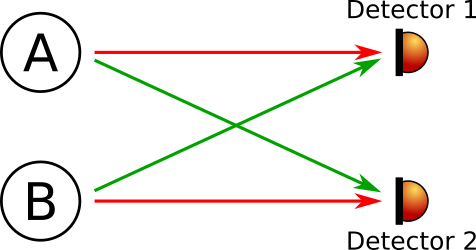
\includegraphics[width=0.55\textwidth]{Fig/Chapter1/HBT_scheme.png}
    \caption{Quantum interpretation of the Hanbury Brown and Twiss effect. For two source points A and B, a joint detection occurs if a photon produced by A is detected in 1 and a photon produced by B is detected in 2 (red arrows), or the other way around A $\rightarrow$ 2 and B $\rightarrow$ 1 (green arrows). Interferences of the paths amplitudes explain the Hanbury Brown and Twiss effect.}
    \label{fig:HBT_scheme}
\end{figure}

At this point we want to underline, as it will be a crucial point in the following of this thesis, that the key ingredient to observe bosonic bunching is the \textbf{chaotic} character of the source. The theoretical development that we have just presented relies on the application of the Central Limit Theorem as the source is made of a large number of independent elementary emitters, each with a random phase. This is notably not the case for laser light that we will discuss in the next paragraph, while giving a rigorous definition of what the term \textbf{chaotic} means.

% This is notably not the case for laser light which is fully coherent and results in $\gtwo (\bm{r}_1,\bm{r}_2)=1$ for all values of $\bm{r}_1$ and $\bm{r}_2$.

To summarize, we have seen in this paragraph an example of a second-order correlation effect, the Hanbury Brown and Twiss effect, and its classical description with a chaotic light source. We also have an insight of how this effect can be understood when considering individual particles, here photons, thus bringing us a bit closer to our goal. The observations of Hanbury Brown and Twiss sparked interest in the community and lead to the development of the new formalism of Quantum Optics \cite{glauber1963quantum} with quantized light fields or light particles, {\it i.e.} photons, with the great success that we know of today. However, we are still overlooking one of the key ingredient of the problem we wish to study, namely \textbf{interactions}. Indeed, photons are essentially mass-less, non-interacting particles. In order to add interactions into these famous quantum optics problems, physicists naturally turned to atoms. As a matter of fact, the quantum optics formalism for photons can be extended quite easily to matter and atoms and gives an incentive to reproduce famous quantum optics effects with massive particles.

We will then take the next step of our journey by looking at the main elements of the theory of Quantum Optics before linking them to atomic physics. This will allow us to understand correlations at the single particle level and to build a bridge between the Optics examples we have described so far and our subject of interest, the study of correlation functions in many-body interacting systems.


\subsection{Second quantization and correlations with individual particles}

The first quantum theories, such as the one developed by Planck to describe black-body radiation, were in fact semi-classical theories in the sense that only the energy of the atoms is quantized, while the radiation fields are still described classically. While semi-classical theories found great success, the observations of Hanbury Brown and Twiss, as well as the development of laser light called for a theory accounting for the corpuscular aspect of light. This gave birth to the Quantum Optics theory whose core element is to push further the idea of quantization by quantizing the radiation fields. While the term is most often associated with atomic physics as we will see later on, we can speak here of \textbf{second quantization}, the first quantization being the one of the energy.

The general idea behind the quantization of the light field is to describe it as a collection of independent quantum harmonic oscillators for the different modes of the field. For a field defined in a box of volume $V=L^3$ with periodic boundary conditions, the field can be described as a superposition of plane waves with a wave vector $k=\frac{2 \pi}{L} n$ with $n \in \N$ each described by a harmonic oscillator \cite{walls2008}:

\begin{equation}
    \hat{\bm{E}}(\bm{r}, t)=\sum_{l} i \bm{\epsilon}_{l} \sqrt{\frac{\hbar \omega_l}{2 \varepsilon_0 V}} \left[e^{i (\bm{k}_{l} \cdot \bm{r} - \omega_l t)} \hat{a}_{l}-e^{-i (\bm{k}_{l} \cdot \bm{r} - \omega_l t)} \hat{a}_{l}^{\dagger}\right]  = \hat{\bm{E}}^{(+)}(\bm{r}, t)+\hat{\bm{E}}^{(-)}(\bm{r}, t)
\end{equation}

\noindent where $\bm{\epsilon}_{l}$ denotes the polarisation of mode $l$. We have introduced the two mutually adjoint operators $\hat{a}_{l}$ and $\hat{a}_{l}^{\dagger}$, analog to the creation and annihilation operators of the quantum harmonic oscillator. In the formalism of the quantum harmonic oscillator, these operators respectively destroy or create a quanta of energy, which in our case corresponds to a photon in mode $l$. Since photons are bosons, $\hat{a}_{l}$ and $\hat{a}_{l}^{\dagger}$ follow the commutation relations:

\begin{equation}
    \left[\hat{a}_{l}, \hat{a}_{l^{\prime}}^{\dagger}\right]=\delta_{l l^{\prime}} \quad\left[\hat{a}_{l^{\prime}}, \hat{a}_{l}\right]=0
\end{equation}

To show the effect of $\hat{a}_{l}$ and $\hat{a}_{l}^{\dagger}$, we introduce the \textbf{number states} or \textbf{Fock states} $\ket{n_l}$, eigenstates of the number operator $\hat{N}_l = \hat{a}_{l}^{\dagger} \hat{a}_{l}$ with $n_l$ representing the number of photons in mode $l$. The Fock state corresponding to the absence of the photons is called the vacuum state and writes $\ket{0}$. The action of the creation and annihilation operators on the Fock states writes:



\begin{equation}
    \hat{a}_{l}^{\dagger} \ket{n_l}=\sqrt{n_l+1}\left|n_l+1\right\rangle
\end{equation}
\begin{equation}
    \hat{a}_{l} \ket{n_l}=\sqrt{n_l}\left|n_l-1\right\rangle
\end{equation}

\noindent From this, we see that every Fock state can be obtained by applying the creation operator on the vacuum state the right amount of times:

\begin{equation}
    \left|n_{l}\right\rangle=\frac{1}{\sqrt{n_{l} !}}\left(\hat{a}_{l}^{\dagger}\right)^{n_{l}}\left|0\right\rangle
\end{equation}


\noindent Finally we can write the Hamiltonian as:

\begin{equation}
    \hat{H}=\sum_{l} \hbar \omega_{l}\left(\hat{N}_{l}+\frac{1}{2}\right)
\end{equation}

\noindent with $\hbar \omega_l$ being the energy of a photon in mode $l$.

\subsubsection{Coherent state and correlation functions}

As we have seen in the last paragraphs, there is a strong connection between correlation functions and the notion of coherence. Motivated by the measurement of cross-correlations between two photodetectors by Hanbury Brown and Twiss, Roy J. Glauber introduced in a very famous paper of 1963 \cite{glauber1963quantum} the notion of $n$-th order coherence in the formalism of Quantum Optics and linked it to $n$-th order correlation functions, as we will see now.

We have talked so far about correlation functions of up to the second order. The concept of correlation functions can be extended to any order $n$ to describe to probability of joint detection of $n$ photons at a set of positions and parameters $\{(\bm{r}_1,t_1),(\bm{r}_2,t_2),...,(\bm{r}_n,t_n)\}$: 

\begin{equation}
    G^{(n)}\left(\bm{r}_{1}, t_{1}, ... , \bm{r}_{n}, t_{n}\right)=\left\langle \hat{\bm{E}}^{(-)}\left(\bm{r}_{1}, t_{1}\right) ... \hat{\bm{E}}^{(-)}\left(\bm{r}_{n}, t_{n}\right) \hat{\bm{E}}^{(+)}\left(\bm{r}_{n}, t_{n}\right) ... \hat{\bm{E}}^{(+)}\left(\bm{r}_{1}, t_{1}\right)\right\rangle
\end{equation}

\label{sec:normal_order}
\noindent Note that the order of the operators is very important with all the terms in $\hat{E}^{(-)}$ and thus $\hat{a}^{\dagger}$ on the left and terms in $\hat{E}^{(+)}$ and thus $\hat{a}$ on the right. This is called \textbf{normal ordering} and ensures that the expectation value of the combination of the operators is zero for the vacuum state. 

Likewise, we introduce the normalized $n-$th order correlation function.

\begin{equation}
    g^{(n)}\left(\bm{r}_{1}, t_{1}, ...,  \bm{r}_{n}, t_{n}\right)=\frac{G^{(n)}\left(\bm{r}_{1}, t_{1}, ...,  \bm{r}_{n}, t_{n}\right)}{\displaystyle \prod_{j=1}^{n} G^{(1)}\left(\bm{r}_{1}, t_{1}, ..., \bm{r}_{n}, t_{n}\right)}
\end{equation}

\noindent From this definition, we define a fully coherent field as a field that verifies, for any value of $n \in \N^*$ \cite{glauber1963quantum}:

\begin{equation}
    g^{(n)}\left(\bm{r}_{1}, t_{1}, ...,  \bm{r}_{n}, t_{n}\right)  = 1
    \label{eq:cond_g_coherent}
\end{equation}

\noindent This means that for a fully coherent field, we have the simple relation:

\begin{equation}
    G^{(j)}\left(\bm{r}_{1}, t_{1}, ... , \bm{r}_{j}, t_{j}\right) = \prod_{i=1}^{j} G^{(j)}(\bm{r}_{i}, t_{i})
    \label{eq:cond_G_coherent}
\end{equation}

Interestingly, we notice that if the field was in a state $\ket{\alpha}$ that would be a ``right'' eigenstate of $\hat{\bm{E}}^{(+)}$, $\hat{\bm{E}}^{(+)} \ket{\alpha} = \alpha \ket{\alpha}$, and a ``left'' eigenstate of $\hat{\bm{E}}^{(-)}$, $\bra{\alpha} \hat{\bm{E}}^{(-)} = \bra{\alpha} \alpha^*$, the conditions \ref{eq:cond_g_coherent} and \ref{eq:cond_G_coherent} would be automatically verified. For simplicity sake, let us consider a single mode field and use the fact that $\hat{\bm{E}}^{(+)} \propto \hat{a}$ and $\hat{\bm{E}}^{(-)} \propto \hat{a}^{\dagger}$. We are thus looking for the state $\ket{\alpha}$ which is an eigenstate of $\hat{a}$. It can be shown that in the basis of the number states, $\ket{\alpha}$ writes \cite{glauber1963coherent}:

\begin{equation}
    |\alpha\rangle=e^{-\frac{1}{2}|\alpha|^{2}} \sum_{n=0}^{\infty} \frac{\alpha^{\mathrm{n}}}{\sqrt{\mathrm{n} !}}|n\rangle
    \label{eq:coherent_state}
\end{equation}

\noindent The state $\ket{\alpha}$ is called a \textbf{coherent state} or Glauber state. We thus find that a coherent state writes as a sum of number states and that the probability to find $n$ photons follows a Poissonian law (see Fig.-\ref{fig:light_statistics}). A well-known example of coherent state is laser light.

\subsubsection{Hanbury Brown and Twiss effect with individual photons}

Let us now close the parenthesis on the coherent state and come back to the Hanbury Brown and Twiss effect described in the last sub-section, characterized by $\gtwo (\bm{r}_1, t_1, \bm{r}_2, t_2) = 2$ for $\bm{r}_1 = \bm{r}_2$ and $t_1=t_2$. As we have just seen, it would by impossible to observe this effect with fully coherent light as $\gtwo (\bm{r}_1, t_1, \bm{r}_2, t_2) = 1$ by definition. Let us rewrite the second order correlation function in the formalism of Quantum Optics to see if it tells us something new. For $\bm{r}_1 = \bm{r}_2$ and $t_1=t_2$, the expression writes: 

\begin{equation}
     g^{(2)}\left(\bm{r}_{1}, t_{1}, \bm{r}_{2}=\bm{r}_1, t_{2}=t_1\right) = \frac{\left\langle\hat{a}^{\dagger} \hat{a}^{\dagger} \hat{a} \hat{a}\right\rangle} {\left\langle\hat{a}^{\dagger} \hat{a}\right\rangle^{2}}
\end{equation}

\noindent Using the commutation relation, we write:

\begin{equation}
    g^{(2)}\left(\bm{r}_{1}, t_{1}, \bm{r}_{2}=\bm{r}_1, t_{2}=t_1\right) = \frac{\left\langle\hat{a}^{\dagger} ( \hat{a} \hat{a}^{\dagger}-1) \hat{a} \right\rangle} {\left\langle\hat{a}^{\dagger} \hat{a}\right\rangle^{2}} = \frac{\mean{N^2}-\mean{N}}{\left\langle\hat{a}^{\dagger} \hat{a}\right\rangle^{2}}  = 1 +  \frac{\sigma^2_N-\mean{N}}{\left\langle\hat{a}^{\dagger} \hat{a}\right\rangle^{2}}
    \label{eq:g2_variance}
\end{equation}

\noindent where we introduce $\sigma_N$ the standard deviation of the number of photons N. We see that the value of the $\gtwo$ function depends on the statistics of the source. For the case of laser light where $N$ follows a Poissonian law, $\sigma_N^2 = \mean{N}$ and we find back $g^{(2)}\left(\bm{r}_{1}, t_{1}, \bm{r}_{2}=\bm{r}_1, t_{2}=t_1\right) = 1$.

To understand how the Hanbury Brown and Twiss effect arises, we need to introduce the concept of \textbf{mixed states}, in opposition to \textbf{pure states}. In some cases, our limited knowledge of the system requires to describe it as a statistical mixture of pure states. This is what we call a mixed state. For such states, we use the formalism of the \textbf{density matrix} which is defined as:

\begin{equation}
    \hat{\rho} = \sum_{i} p_i \ket{\Psi_i} \bra{\Psi_i}
\end{equation}

\noindent where $p_i$ is the probability for the system to be in the pure state $\ket{\Psi_i}$. The expectation value of an operator $\hat{O}$ is obtained through:

\begin{equation}
    \mean{\hat{O}} = \rm{Tr}(\hat{\rho} \hat{O})
\end{equation}

\begin{figure}
    \centering
    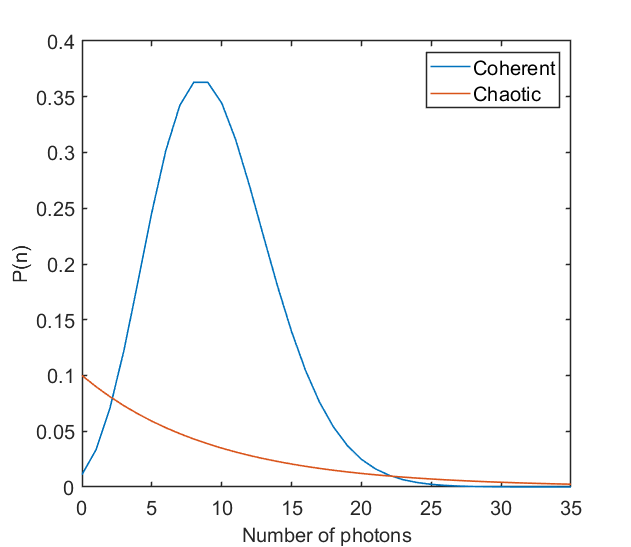
\includegraphics[width=0.7\textwidth]{Fig/Chapter1/coherent_vs_chaotic.png}
    \caption{Probability distribution for the number of photons for coherent and chaotic light sources for a fixed value of $|\alpha^2|$.}
    \label{fig:light_statistics}
\end{figure}

This is formalism is particularly useful to describe light sources made of a large number of independent individual emitters. Let us say that the first emitter brings the field in state $\ket{\alpha_1}$, the second emitter in state $\ket{\alpha_2}$ etc.. It can be shown (\cite{glauber1963coherent}) that for a large number of individual emitters $j$, the probability distribution for the complex amplitude $\alpha=\alpha_1 + \alpha_2 + ... + \alpha_j$ follows a Gaussian law:

\begin{equation}
    P(\alpha)= \frac{1}{\pi \mean{n}} e^{-\frac{|\alpha|^2}{\mean{n}}}
    \label{eq:p_alpha}
\end{equation}

\noindent where $\mean{n}$ is the mean value of $|\alpha|^2$ and represents the number of number of energy quanta in the mode. From this, we use equation \ref{eq:coherent_state} to write the density matrix of the system in the basis of the number states:

\begin{equation}
    \hat{\rho}=\frac{1}{1+\langle n\rangle} \sum_{m=0}^{\infty}\left(\frac{\langle n\rangle}{1+\langle n\rangle}\right)^{m}|m\rangle\langle m|
    \label{eq:rho_chaotic}
\end{equation}

\noindent The probability to find $m$ photons then writes (see Fig.-\ref{fig:light_statistics}):

\begin{equation}
    P(m)=\frac{1}{1+\langle n\rangle}\left(\frac{\langle n\rangle}{1+\langle n\rangle}\right)^{m}
    \label{eq:chaotic_light}
\end{equation}


\noindent A light source with these statistics is called a \textbf{chaotic} light source. This is notably the case of thermal light, described by the Planck's distribution with $\mean{n}=1/(e^{h\nu/\kB T}-1)$. From equation \ref{eq:chaotic_light}, we show that the variance of the photon number $N$ writes:

\begin{equation}
    \sigma_N^2=\mean{N}^2+\mean{N}
\end{equation}

\noindent Injecting this result into equation \ref{eq:g2_variance}, we find that for a chaotic light source, \\ $g^{(2)}\left(\bm{r}_{1}, t_{1}, \bm{r}_{2}, t_{2}\right)=2$ for $\bm{r}_{1}=\bm{r}_{2}$ and $t_1=t_2$, the bosonic bunching observed by Hanbury Brown and Twiss!



% For chaotic thermal light, the photons statistics are set by the Bose-Einstein statistics giving $\sigma_N^2=\mean{N}^2+\mean{N}$, we find back $g^{(2)}=2$! On the other hand, for the coherent light of a laser, the standard deviation of the photon number is set by the shot noise $\sigma_N^2=N$ and we retrieve $g^{(2)}=1$.

In fact, this result can be obtained through a complementary approach that relies on the application of the Wick's theorem \cite{gardiner2000quantum}.

\begin{tcolorbox}[colback=red!5!white,colframe=red!75!black,title=\textbf{Wick's theorem}]
\label{sec:wick}
When a system is characterized by a Gaussian density matrix $\hat{\rho} \propto \exp(\sum_i \gamma_i \hat{a}_i^{\dagger} \hat{a}_i)$, the high-order products of of creation and annihilation operators can be factorized into all possible products of only two operators. For bosonic particles, this writes:

$$ \mean{\hat{A}_1 ... \hat{A}_{2m}} = \sum_{\sigma} \mean{\hat{A}_{i_1} \hat{A}_{i_2}} \mean{\hat{A}_{i_3} \hat{A}_{i_4}} ... \mean{\hat{A}_{i_{2m-1}} \hat{A}_{i_{2m}}}$$

where $\sigma$ denotes all possible permutations changing the order $1,2,...,2m$ to $i_1,i_2,...,i_{2m}$, and $\hat{A}_i$ is any creation or annihilation operator.

\end{tcolorbox}

As shown in equations \ref{eq:p_alpha} and \ref{eq:rho_chaotic}, the density matrix of a chaotic light source is Gaussian, it is therefore possible to use Wick's theorem to simplify the second-order correlation function exactly as we did classically in \ref{sec:hbt_classical} :

\begin{equation}
    \gtwo \left(\bm{r}_{1}, t_{1}, \bm{r}_{2}, t_{2}\right) = 1 + |g^{(1)}\left(\bm{r}_{1}, t_{1}, \bm{r}_{2}, t_{2}\right)|^2
\end{equation}

\noindent As $g^{(1)}\left(\bm{r}_{1}, t_{1}, \bm{r}_{2}, t_{2}\right)=1$ for $\bm{r}_1=\bm{r}_2$ and $t_1=t_2$, we find back that $\gtwo \left(\bm{r}_{1}, t_{1}, \bm{r}_{2}, t_{2}\right)=2$ for $\bm{r}_1=\bm{r}_2$ and $t_1=t_2$. Actually, this procedure can be extended up to any order to show that the $n$-th order correlation function can be simplified to a linear combination of first order correlation functions. This means that the entirety of the information is contained in the first order correlation function. The normalized probability of joint detection of $n$ photons then writes:

\begin{equation}
    g^{(n)} (\bm{r}_1,...,\bm{r}_n,t_1,...,t_n) = n! \ \mathrm{for} \ \bm{r}_1=\bm{r}_2= ... =\bm{r}_n \ \mathrm{and} \ t_1=t_2=...=t_n
\end{equation}

\noindent which is a generalisation of the two particles bosonic bunching, seen previously, for $n$ particles. On a side note, notice that Wick's theorem does not apply to laser light as the density matrix describing it is not Gaussian.

We have thus seen how the Hanbury Brown and Twiss effect writes in the formalism of Quantum Optics and shown the differences between a coherent and chaotic light source. We will keep this result in the back of our minds as it will be of primary importance when we will study second order correlation functions with interacting atoms a little further down the line.



\section{Bogoliubov theory of the weakly-interacting gas}

Thus far, we have familiarized ourselves with correlation functions and seen through a few examples of Optics the kind of information they contain, with both classical and quantum formalisms. We will now try to use this tool to study one of the most simple many-body problem, the weakly-interacting homogeneous Bose gas, {\it i.e.} an ensemble of bosonic particles with weak contact interactions in a box of volume $V$. This system is a nice compromise: while we account for interactions between individual particles and might then observe interesting correlations phenomena, the system can still be described theoretically at the price of a few approximations. This theory has been developed by Nikolay Bogoliubov in his famous 1947 article \cite{bogoliubov1947}. In this section, we will remind the main lines of Bogoliubov's approach and see what it tells us in terms of correlation functions.

\subsection{Second quantization in atomic physics}

Before diving into the specifics of Bogoliubov theory, we briefly remind the formalism of second quantization in atomic physics that will allow us to use the results obtained in the last paragraph for Quantum Optics. Interestingly, the idea of second quantization of Quantum Optics can be extended to treat the quantum many-body problem in a more efficient and intuitive way. Indeed, calculations get quite complex when considering many-body systems of indistinguishable particles as the many-body wave-function must be (anti-)symmetrized, a problem that the second quantization formalism aims to resolve.

The key point is to switch things around by counting the number of particles in each state instead of the usual approach which would be to determine in which state each particle is. To this end, the many-body state is represented as set of occupation numbers:

\begin{equation}
   \ket{ \{n_{\alpha}\}} = \ket{n_1,n_2,...,n_{\alpha},...}
\end{equation}

\noindent where $n_{\alpha}$ denotes the number of particles in state $\alpha$. For fermions, this number is either 0 or 1 because of the Pauli exclusion principle, whereas it can be any integer value for bosons. We recognize the states $\ket{ \{n_{\alpha}\}}$ as the \textbf{Fock states} described in the last paragraph. As for Quantum Optics, we introduce creation and annihilation operators $\hat{a}^{\dagger}_{\alpha}$ and $\hat{a}_{\alpha}$ respectively creating or destroying a particle in state $\alpha$. For bosons on which this thesis will be focused:

\begin{equation}
    \hat{a}_{\alpha}^{\dagger} \ket{n_{\alpha}}=\sqrt{n_{\alpha}+1}\left|n_{\alpha}+1\right\rangle
\end{equation}
\begin{equation}
    \hat{a}_{\alpha} \ket{n_{\alpha}}=\sqrt{n_{\alpha}}\left|n_{\alpha}-1\right\rangle
\end{equation}

Just as for photons, the Fock states are constructed by applying the creation operators the right amount of times on the vacuum state. For bosonic particles, the commutation relation is the same as for photons:

\begin{equation}
    \left[\hat{a}_{\alpha}, \hat{a}_{\alpha^{\prime}}^{\dagger}\right]=\delta_{\alpha \alpha^{\prime}} \quad\left[\hat{a}_{\alpha^{\prime}}, \hat{a}_{\alpha}\right]=0
\end{equation}

\noindent This has the advantage that the symmetric properties are taken care of by the commutation relations, avoiding complex symmetrization calculation. 

% This formalism is thus very close to the one we have developed for Quantum Optics. We will thus be able to use with atoms the results on second-order correlation functions presented earlier for photons, while adding interactions to the mix to make things more interesting.

\subsection{Bogoliubov approximation}

% \NOTE{Etapes avant?}

We now go back to the problem of the weakly-interacting Bose gas with contact interactions. In the second quantization formalism, the Hamiltonian of the system writes:

\begin{equation}
    \hat{H}=\sum_{\bm{k}}\frac{\hbar^2 k^2}{2m} \hat{a}^{\dagger}_{\bm{k}}  \hat{a}_{\bm{k}} +  \frac{g}{2V} \sum_{\bm{k}_1,\bm{k}_2,\bm{k}_3} \hat{a}^{\dagger}_{\bm{k_1}+\bm{k_3}} \hat{a}^{\dagger}_{\bm{k_2}-\bm{k_3}} \hat{a}_{\bm{k_1}} \hat{a}_{\bm{k_2}} 
\end{equation}

\noindent where $g=\dfrac{4 \pi \hbar^2 a_s}{m}$ is the strength of the interactions with $a_s$ the s-wave sacttering length. The approximation of contact interactions is reasonable in the case where the scattering length is much smaller than the distance between atoms, $|a| n^{1/3} \ll 1$, as it is the case in our experiment. In order to simplify this Hamiltonian, we use the Bogoliubov approximation that relies on two points:

\begin{itemize}
    \item Since the interactions are weak, we assume that the number of atoms outside of the BEC is small. We therefore only consider interaction processes removing two particles from the BEC or bringing back two particles into the BEC. Mathematically speaking, we drop all terms higher than quadratic in $\hat{a}_{\bm{k}}$ and $\hat{a}^{\dagger}_{\bm{k}}$.
    \item The number of atoms $\NBEC$ is assumed to be very large. Therefore, we replace $\hat{a}_{\bm{0}}$ and $\hat{a}^{\dagger}_{\bm{0}}$ by $\sqrt{\NBEC}$. 
\end{itemize}

\noindent With these approximations, the simplified Hamiltonian writes:

\begin{equation}
    H_{\rm{bogo}}=\sum_{\bm{k}}\frac{\hbar^2 k^2}{2m} \hat{a}^{\dagger}_{\bm{k}}  \hat{a}_{\bm{k}} +  \frac{gn}{2} \sum_{\bm{k}} (\hat{a}^{\dagger}_{\bm{k}} \hat{a}^{\dagger}_{-\bm{k}} +\hat{a}_{\bm{k}} \hat{a}_{-\bm{k}})+\frac{gn\NBEC}{2}
\end{equation}

\noindent with $n=\NBEC/V$. We now want to diagonalize the Hamiltonian. This is achieved through the linear Bogoliubov transformation where we introduce a new operator:

\begin{equation}
    \hat{b}_{\bm{k}}=u_{\bm{k}} \hat{a}_{\bm{k}} + v_{-\bm{k}} \hat{a}^{\dagger}_{-\bm{k}}
\end{equation}

\noindent To determine the expression of the coefficients $u_{\bm{k}}$ and $v_{\bm{k}}$, we impose that the new operator $\hat{b}_{\bm{k}}$ follows the bosonic operator commutation rule:

\begin{equation}
    [\hat{b}_{\bm{k}},\hat{b}^{\dagger}_{\bm{k}'}]= \delta_{\bm{k},\bm{k}'}
\end{equation}

\noindent This gives $u_{\bm{k}}^2 -  v_{-\bm{k}}^2 =1$. We can therefore write $u_{\bm{k}}={\rm cosh}(\alpha_{\bm{k}})$ and $v_{-\bm{k}}={\rm sinh}(\alpha_{\bm{k}})$ and look to determine $\alpha_{\bm{k}}$. This value must be chosen so that the coefficients of the terms in $\hat{b}^{\dagger}_{\bm{k}} \hat{b}^{\dagger}_{-\bm{k}}$ and $\hat{b}_{\bm{k}} \hat{b}_{-\bm{k}}$ vanish. We obtain an additional equation:

\begin{equation}
    \frac{g n}{2}\left(u_{\bm{k}}^{2}+v_{-\bm{k}}^{2}\right)+\left(\frac{k^{2}}{2 m}+g n\right) u_{\bm{k}} v_{-\bm{k}}=0
\end{equation}

\noindent from which we finally obtain after a few calculations using the properties of hyperbolic functions:

\begin{equation}
    u_{\bm{k}}, v_{-\bm{k}}=\pm\left(\frac{\hbar^2k^{2} / 2 m+g n}{2 \varepsilon(k)} \pm \frac{1}{2}\right)^{1 / 2}
\end{equation}

\noindent with 

\begin{equation}
    \varepsilon(k)=\sqrt{\frac{\hbar^2 k^2}{2m}\left(\frac{\hbar^2 k^2}{2m}+2gn \right)}
\end{equation}

\noindent the famous Bogoliubov dispersion relation. The Hamiltonian has now been diagonalized and writes:

\begin{equation}
    \hat{H}_B = \sum_{\bm{k}}\varepsilon(k) \hat{b}^{\dagger}_{\bm{k}}  \hat{b}_{\bm{k}}+E_0
\end{equation}

\noindent The system of interacting particles has thus been transformed into a system of non-interacting Bogoliubov quasi-particles associated to creation and annihilation operators $\hat{b}^{\dagger}_{\bm{k}}$ and $\hat{b}_{\bm{k}}$ with a dispersion relation $\varepsilon(k)$. The prediction of this excitation spectrum is one of the key results of Bogoliubov theory that we will now discuss in further details.

\subsection{Spectrum of excitations}
\label{sec:spectrum}

The Bogoliubov dispersion relation has two clear asymptotic trends for small and high momentum values. For low values of $k$, using $\frac{\hbar^2 k^2}{2m} \ll 2gn$, we obtain:

\begin{equation}
    \varepsilon(k) \underrel{k \to 0}{=} \hbar k \sqrt{\frac{gn}{m}}
\end{equation}

\noindent The dispersion relation takes a phonon-like linear dispersion form where the sound velocity is $c=\sqrt{\dfrac{gn}{m}}$. In this regime, the Bogoliubov quasi-particles are thus phonons that can be seen as a coherent superposition of a forward and backward propagating real particles $\hat{b}_{\bm{k}}=u_{\bm{k}} \hat{a}_{\bm{k}} + v_{-\bm{k}} \hat{a}^{\dagger}_{-\bm{k}}$ with $\abs{u_{\bm{k}}} \simeq \abs{v_{-\bm{k}}}$.

On the other hand, at high values of $k$, the dispersion relation becomes the one of free particles:

\begin{equation}
    \varepsilon(k) \underrel{k \to +\infty}{=} \frac{\hbar^2 k^2}{2m}
\end{equation}

\noindent In terms of operators, $v_k \underrel[c]{k \to +\infty}{=} 0$ and $u_k \underrel[c]{k \to +\infty}{=} 1$ so $\hat{b}_{\bm{k}}\underrel[c]{k \to +\infty}{=}\hat{a}_{\bm{k}}$, a quasi-particle is equivalent to a real particle. 

The transition between the two regimes occurs when $\frac{\hbar^2 k^2}{2m} \simeq gn$, it thus convenient to define a characteristic length associated to this momentum range:

\begin{equation}
    \xi = \sqrt{\frac{\hbar^2}{2mgn}}
\end{equation}

\noindent This length is called the \textbf{healing length}. Its name comes from the fact the $\xi$ represent the length scale on which a local perturbation of the density is ``healed'' back to the bulk density.

%We will use it later when discussing our experimental results to characterize the region of the Bogoliubov spectrum we are probing.

The Bogoliubov spectrum of excitations has been a very successful theoretical prediction observed experimentally in a large variety of systems \cite{fontaine2018,miller1962,ozeri2005,steinhauer2002excitation,stepanov2019}. This is not however all that is predicted by Bogoliubov theory. As we will now see, this theory can also be used to understand the \textbf{ground-state} of the system.

\begin{figure}
    \centering
    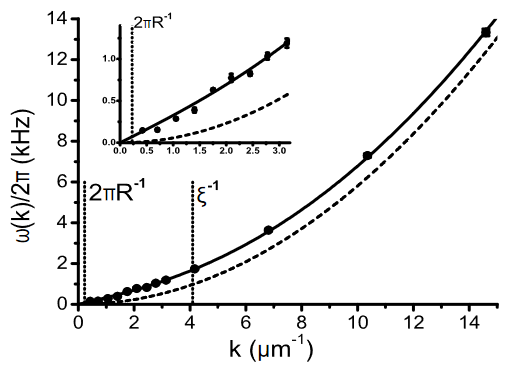
\includegraphics[width=0.65\textwidth]{Fig/Chapter1/bogo_steinhauer.png}
    \caption{Experimental observation of the Bogoliubov excitation spectrum (Steinhauer {\it et al.} \cite{steinhauer2002excitation}). The phononic and free particle parts are clearly identifiable. The inset shows a zoom on the linear part of the spectrum and the dashed line the free particle spectrum. $\xi$ is the healing length of the condensate.}
    \label{fig:my_label}
\end{figure}

\subsection{Many-body ground state and quantum depletion}

\label{sec:many_body_ground_state}

As we have just seen, the Bogoliubov approach describes the weakly-interacting Bose gas excitations as non-interacting quasi-particles. They therefore behave as ideal bosons and follow the Bose distribution:

\begin{equation}
    \langle b^{\dagger}_{\bm{k}}  b_{\bm{k}} \rangle=\frac{1}{e^{-\varepsilon(k)/(k_B T)}-1} 
    \label{eq:bose_qp}
\end{equation}

\noindent Naturally, at $T=0$, the population of quasi-particles is null: $\langle \hat{b}^{\dagger}_{\bm{k}}  \hat{b}_{\bm{k}} \rangle_{T=0}=0$. That being said, let us now write the population of real particles for a given momentum $k \neq 0$:

\begin{equation}
    \langle \hat{a}^{\dagger}_{\bm{k}}  \hat{a}_{\bm{k}} \rangle=\textcolor{blue}{(|u_k|^2+|v_k|^2)\langle \hat{b}^{\dagger}_{\bm{k}}  \hat{b}_{\bm{k}} \rangle} + \textcolor{green}{|v_k|^2}
\end{equation}

\noindent The blue term corresponds to the Bogoliubov excitations populated by temperature. We will call the fraction of particles removed from the condensate this way the \textcolor{blue}{\textbf{thermal depletion}}. This fraction vanishes at $T=0$. Very interestingly, we see the apparition of an additional term \textcolor{green}{$|v_k|^2$} that results from the non commutation of the bosonic creation and annihilation operators, the signature of an essentially quantum phenomenon. This term tells us that $\langle \hat{a}^{\dagger}_{\bm{k}}  \hat{a}_{\bm{k}} \rangle_{T=0} \neq 0$, meaning that there are some atoms outside of the BEC with a non zero momentum in the ground state! Under the interplay between interactions and quantum fluctuations, some atoms are removed from the BEC and obtain a non zero momentum. The fraction of these atoms is called the \textcolor{green}{\textbf{quantum depletion}}. 

We are thus looking at a system which falls into our general area of interest described in the introduction of this thesis, namely many-body systems with interactions displaying quantum behaviors. The weakly-interacting Bose gas shows the advantage to be one of the conceptually simplest many-body systems for which a theory can be derived as we just have shown. As explained in the beginning of this chapter, many-body systems are often efficiently characterized by correlation functions. Let us now discuss what are the relevant correlation functions to study for the weakly-interacting Bose gas.


\section{Two-body correlations in the weakly-interacting Bose gas}

\subsection{Pairing mechanism in the quantum depletion}

We have seen in the last paragraph the mathematical approach that reveal the existence of the quantum depletion, but that seems hard to grasp in a physical manner. We therefore now look to build a microscopical, physically meaningful picture of how the quantum depletion emerges. We remind that a key ingredient of the Bogoliubov theory is that the only considered interaction processes are the ones involving two particles of the BEC or two particles outside of the BEC being brought into it. From this consideration, we understand that the atoms belonging to the quantum depletion were initially in the BEC and were removed from it after undergoing a two-body interaction process. The interaction process populating the quantum depletion thus involves two atoms in the BEC with a momentum $k \simeq 0$. To conserve the overall momentum, the two atoms leaving the BEC then have opposite momenta $\bm{k}$ and $-\bm{k}$ and form a momentum correlated pair. This falls exactly into the kind of signal we are interested in, namely correlations between several particles, here two, caused by a quantum, interaction-induced effect.

\begin{figure}
    \centering
    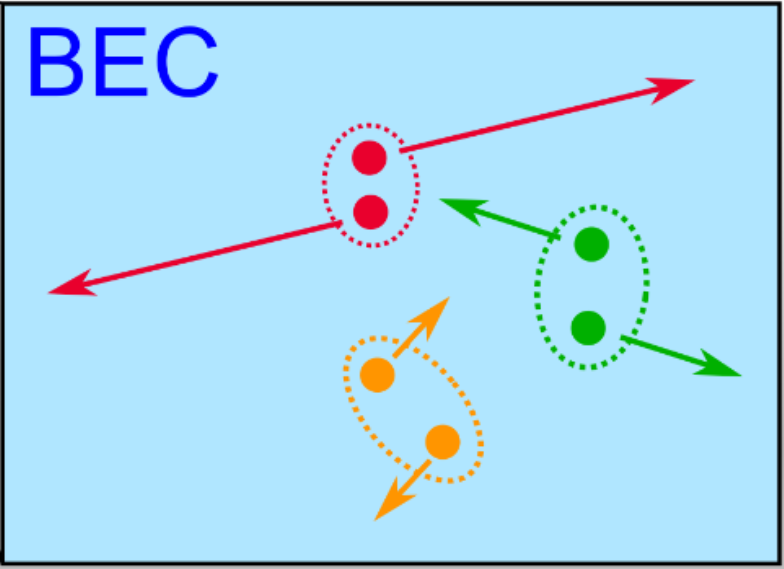
\includegraphics[width=0.5\textwidth]{Fig/Chapter1/pairs.png}
    \caption{Illustration of the \kmk pairing of the quantum depleted atoms in the BEC (light blue).}
    \label{fig:bec_pairs}
\end{figure}

The common factor with quantum effects is that they usually defy our intuition built on our observation of the everyday world, well described by classical physics. In this case, the ``quantum weirdness'' comes from the fact this process seems to violate the conservation of energy: the two at atoms initially \textbf{at rest} each have an extra kinetic energy $\frac{\hbar^2 k^2}{2m}$ after the interaction process, giving them the $\bm{k}$ and $-\bm{k}$ momenta. Naturally, the conservation of energy is still well respected here. The apparent contradiction comes from the fact that it is conceptually wrong to isolate two atoms in the BEC. The ground-state must rather be understood as a single many-body wave-function describing indistinguishable atoms, with a non zero component for momentum values $k \neq 0$. The energy of the many-body ground state of the weakly-interacting Bose gas contains a small correction that corresponds to the presence of the \kmk pairs of the quantum depletion. This small correction is called the Lee-Huang-Yang correction, named after the authors of the seminal 1957 article \cite{lee1957} that first predicted the presence of the \kmk pairs. While they have already been experimental studies confirming the presence of quantum depleted atoms with large momentum \cite{sokol1995,xu2006} and the prediction of the quantum depleted fraction \cite{lopes2017}, the \kmk correlations in the ground-state have not yet been observed.

The fascinating aspect of this \kmk pairing effect is that it occurs in an \textbf{at-equilibrium} system and therefore can only result from the effect of quantum fluctuations. Although we cannot draw a rigorous direct analogy, this kind of effect is reminiscent of other puzzling phenomenon such as Hawking radiation \cite{hawking1974} describing the evaporation of black holes where a pair of correlated photons is produced near the event horizon, or the creation of particle/anti-particle pairs from the vacuum. By studying this \kmk correlation signal, we can therefore study how quantum correlations and possibly entanglement emerges in at-equilibrium quantum many-body systems from the interplay between quantum fluctuations and interactions, which constitutes an exciting prospect that will be the principal motivation of this thesis.





\subsection{Second order correlation functions within Bogoliubov theory}

\label{sec:2nd_order_bogo}

Now that we have identified the \kmk pairing mechanism in the quantum depletion, it is natural to look for a signature of it in the second order correlation function that characterizes the correlations between two particles. We start by describing the general case of the two-body correlator between two modes $\bm{k}$ and $\bm{k'}$:

\begin{equation}
    G(\bm{k},\bm{k}')=\langle \hat{a}^{\dagger}_{\bm{k}} \hat{a}^{\dagger}_{\bm k'} \hat{a}_{\bm k} \hat{a}_{\bm {k}'} \rangle
\end{equation}

As we have seen in the previous section, the Bogoliubov Hamiltonian is diagonal in the quasi-particle basis. All quantum states thus have Gaussian statistics, allowing us to use Wick's theorem (see \ref{sec:wick}) to simplify the correlator:

\begin{equation}
    G(\bm{k},\bm{k}')=\langle \hat{a}^{\dagger}_{\bm k} \hat{a}^{\dagger}_{\bm {k}'} \rangle \mean{\hat{a}_{\bm k} \hat{a}_{\bm {k}'}} + \langle \hat{a}^{\dagger}_{\bm k} \hat{a}_{\bm k} \rangle \langle \hat{a}^{\dagger}_{\bm {k}'} \hat{a}_{\bm {k}'} \rangle + \langle \hat{a}^{\dagger}_{\bm k} \hat{a}_{\bm {k}'} \rangle \langle \hat{a}^{\dagger}_{\bm {k}'} \hat{a}_{\bm k} \rangle
    \label{eq:wick_bogo}
\end{equation}

We end up with three different terms:

\begin{itemize}
    \item The first term equals $| \langle \hat{a}^{\dagger}_{\bm k} \hat{a}^{\dagger}_{\bm {k}'} \rangle |^2$ and is non zero only when $\bm{k}'=-\bm{k}$. This corresponds to the \kmk correlations.
    \item We recognize in the second term the product of the momentum densities $\rho(\bm{k}) \rho(\bm{k}')$.
    \item The third term equals $| \langle \hat{a}^{\dagger}_{\bm k} \hat{a}_{\bm {k}'} \rangle |^2$ and is non zero only when $\bm{k}'=\bm{k}$. This correspond to the Hanbury Brown and Twiss effect or bosonic bunching described earlier.
\end{itemize}

\noindent We regroup the two last terms in the function $G^{(2)}_{N}({\bm k},{\bm k}')= \rho({\bm k})\rho({\bm k}') + | \langle \hat{a}^{\dagger}_{\bm k} \hat{a}_{\bm {k}'} \rangle |^2$ that we call the \textbf{normal} correlation function as the operators are normally ordered (see \ref{sec:normal_order}). In opposition, we introduce for the last term the function $G^{(2)}_{A}({\bm k},{\bm k}')=| \langle \hat{a}^{\dagger}_{\bm k} \hat{a}^{\dagger}_{\bm {k}'} \rangle |^2 $ that we call the \textbf{anomalous} correlation function. Interestingly, this term is non zero only if there exists interactions coupling different modes, in our case $\bm{k}$ and $-\bm{k}$.

We must now determine which atoms participate to which correlation signal. We have seen in \ref{sec:many_body_ground_state} that the depletion of the condensate is divided between the \textbf{quantum} and the \textbf{thermal} depletion. As we have shown in the last sub-section, we expect that the quantum depleted atoms contribute to the anomalous \kmk correlation signal due to the microscopic mechanism describing how the quantum depletion is populated. In fact, it is also possible for the thermal depletion to contribute to the anomalous correlation signal. Indeed, as discussed in \ref{sec:spectrum}, for low $k$ values such as $k \xi \ll 1$, the Bogoliubov quasi-particles have a strong phononic character $\hat{b}_{\bm{k}}=u_{\bm{k}} \hat{a}_{\bm{k}} + v_{-\bm{k}} \hat{a}^{\dagger}_{-\bm{k}}$ with $\abs{u_{\bm{k}}} \simeq \abs{v_{-\bm{k}}}$. This means that we have \kmk correlations in terms of real particles. This feature goes against our goal which is to study the quantum coherences of the many-body ground state, as we understand that if we were to observe \kmk correlations, we would not be able to unambiguously attribute them to the quantum depletion as they could come from phonons of the thermal depletion. However, we saw in \ref{sec:spectrum} that the phononic character of the excitations disappears for high $k$ values such as $k\xi \geq 1$. This gives us a nice workaround: if we restrict our measurement of \kmk correlations to high $k$, we could safely attribute them to the quantum depletion.

Let us now take a look at normal correlations, \ie bosonic bunching. As we have seen in \ref{sec:spectrum} and \ref{sec:many_body_ground_state}, the Bogoliubov quasi-particles of the thermal depletion follow the Bose distribution and therefore have thermal chaotic statistics. This qualifies the thermal depletion to show bosonic bunching. On the other hand, the \kmk pairs of the quantum depletion form a pure quantum state for which we would then not expect bosonic bunching. The situation is however a bit more subtle than that. Indeed, when we look for local \kk correlations, we do so between atoms belonging to two different pairs. To compute the density matrix describing these atoms, we therefore trace over the second atom of the pair that we ignore, retrieving a density matrix with a chaotic character \cite{yurke1987} as we will illustrate in the next paragraph. This means that we should observe bosonic bunching with the quantum depletion as well!

% Nonetheless, this low $k$ region corresponds more or less to the region that will need to be removed to exclude the BEC from the analysis (experimental numbers will be given in Chapter 4). We therefore do not have to care for the contribution of the thermal depletion to the \kmk correlation signal that will in our case only reflect the quantum depletion correlations.

In a nutshell, we have two correlation functions of interest well separated in momentum space and containing very different types of information. On the one hand, the normal correlations correspond to close-by correlations and bosonic bunching revealing the chaotic statistics of the system, coming from either the thermal statistics of the thermal depletion, or the partial trace over the second atom of the pair destroying the quantum coherence for the quantum depletion. On the other hand, the anomalous correlations correspond to \kmk correlations and reveal the quantum coherences of the many-body ground state, provided that we probe them in the high $k$ region. While our main goal will be to measure the anomalous \kmk correlations for the reasons mentioned earlier, it will also be of great interest to measure the local normal correlations to contrast their behaviour with the anomalous correlations as a mean to illustrate the different physical origins of the two signals. 


\subsection{Characterization of the anomalous correlation function : analogy with the non-degenerate parametric amplifier}

\label{sec:amp_parametric}

We now look to further theoretically characterize the anomalous correlation function within the frame of the Bogoliubov theory. The idea is to identify some key features of the anomalous correlation signal to look for in the experiment. To begin, let us go back to the simplified Bogoliubov Hamiltonian before its diagonalisation.

\begin{equation}
    H_{\rm{bogo}}=\sum_{\bm{k}}\frac{\hbar^2 k^2}{2m} \hat{a}^{\dagger}_{\bm{k}}  \hat{a}_{\bm{k}} +  \frac{gn}{2} \sum_{\bm{k}} (\hat{a}^{\dagger}_{\bm{k}} \hat{a}^{\dagger}_{-\bm{k}} +\hat{a}_{\bm{k}} \hat{a}_{-\bm{k}})+\frac{gn\NBEC}{2}
\end{equation}


\noindent For simplicity sake, let's consider that there are only two modes, $\bm{k}$ and $-\bm{k}$  : 

\begin{equation}
        H_{\rm{bogo}}'=\frac{\hbar^2 k^2}{2m} (\hat{a}^{\dagger}_{\bm{k}}  \hat{a}_{\bm{k}} + \hat{a}^{\dagger}_{-\bm{k}}  \hat{a}_{-\bm{k}}) +  \frac{gn}{2}  (\hat{a}^{\dagger}_{\bm{k}} \hat{a}^{\dagger}_{-\bm{k}} +\hat{a}_{\bm{k}} \hat{a}_{-\bm{k}})+\frac{gn\NBEC}{2}
\end{equation}

\noindent As it is now the custom, we look towards Optics for help as we recognize that the Hamiltonian is of the same form of the well-known problem of the non-degenerate parametric amplifier. This describes a non-linear Optics effect where a pump photon at frequency $2 \omega$ interacts with a non-linear optical medium to produce photons in two modes at frequency $\omega_1$ and $\omega_2$, the signal and idler mode, with $2 \omega = \omega_1 + \omega_2$. The Hamiltonian of the system is \cite{walls2008}:

\begin{equation}
    H=\hbar \omega_1 \hat{a}_1^{\dagger} \hat{a}_1+ \hbar \omega_2 \hat{a}_2^{\dagger} \hat{a}_2 + i \hbar \chi (\hat{a}_1^{\dagger}  \hat{a}_2^{\dagger} e^{-2i\omega t} - \hat{a}_1 \hat{a}_2 e^{2i\omega t})
\end{equation}

\noindent where $\chi$ is a coupling constant. We thus have a direct analogy with the weakly-interacting Bose gas, the modes 1 and 2 being the analogues of the momentum modes $\bm{k}$ and $-\bm{k}$. This comparison does not come out of the blue as this system was used in landmark experiments \cite{burnham1970,heidmann1987observation} to demonstrate important results of quantum mechanics that were later reproduced with pairs of atoms instead of pairs of photons \cite{bucker2011,dall2009paired,perrin2007observation}. As we will now see, these observations also applies for the \kmk pairs of the quantum depletion that we wish to study. Let us then present the theoretical treatment of the non-degenerate parametric amplifier and see what it tells us about our system of interest \cite{hodgman2017solving}. 

This time-dependent problem is best solved in the interaction picture, {\it i.e.} where the time dependence is carried by both operators and states. The interaction Hamiltonian then writes:

\begin{equation}
    H_I=i \hbar \chi (\hat{a}_1^{\dagger}  \hat{a}_2^{\dagger} - \hat{a}_1 \hat{a}_2)
\end{equation}

\noindent The counterpart to the Schrödinger equation in the interaction picture is the Heisenberg equation of motion:

\begin{equation}
    \frac{\mathrm{d}\hat{a}_1}{\mathrm{d}t}= \frac{1}{i\hbar} [\hat{a}_1,H_I]=\chi \hat{a}_2^{\dagger}
\end{equation}
\begin{equation}
    \frac{\mathrm{d}\hat{a}_2^{\dagger}}{\mathrm{d}t}= \frac{1}{i\hbar} [\hat{a}_2^{\dagger},H_I]=\chi \hat{a}_1
\end{equation}

\noindent The solution of these coupled equations are:

\begin{equation}
    \hat{a}_1(t)=\hat{a}_1(0) \mathrm{cosh} \chi t + \hat{a}_2^{\dagger}(0) \rm{sinh} \chi t
    \label{eq:a1}
\end{equation}
\begin{equation}
    \hat{a}_2(t)=\hat{a}_2(0) \mathrm{cosh} \chi t + \hat{a}_1^{\dagger}(0) \rm{sinh} \chi t
    \label{eq:a2}
\end{equation}

\noindent From this, we can derive a few interesting results. First, we write the quantum state $\ket{\Psi(t)}$ generated by the parametric amplification process. To do so, we write the interaction picture evolution operator:

\begin{equation}
    \hat{U}(t)=\exp \left[\chi t\left(\hat{a}_{1}^{\dagger} \hat{a}_{2}^{\dagger}+\hat{a}_{1} \hat{a}_{2}\right)\right]
\end{equation}

\noindent At the price of a few lines of calculations (see \cite{schumaker1985new}), this operator can be re-written in a factored form:

\begin{equation}
    \hat{U}(t)=\frac{1}{(\cosh \chi t)} e^{\hat{a}_{1}^{\dagger} \hat{a}_{2}^{\dagger} \tanh \chi t} e^{-\left(\hat{a}_{1}^{\dagger} \hat{a}_{1}+\hat{a}_{2}^{\dagger} \hat{a}_{2}+1\right) \ln (\cosh \chi t)} e^{-\hat{a}_{1} \hat{a}_{2} \tanh \chi t}
\end{equation}

\noindent While this expression is a bit daunting, it becomes way simpler if we consider the initial state to be the vacuum:

\begin{equation}
    \ket{\Psi(t)} = \frac{1}{(\cosh \chi t)} e^{\hat{a}_{1}^{\dagger} \hat{a}_{2}^{\dagger} \tanh \chi t} \ket{0}
\end{equation}

\noindent We obtain easily from this the expression of $\ket{\Psi(t)}$ in the number states basis:

\begin{equation}
    |\Psi(t)\rangle=\frac{1}{(\cosh \chi t)} \sum_{n=0}^{\infty}(\tanh \chi t)^{n} \ket{n}_1 \ket{n}_2
\end{equation}

\label{sec:correlated_pop}

\noindent The state thus writes as a superposition of number states with the same number of photons in modes 1 and 2. The populations in modes 1 and 2 are therefore perfectly correlated, a feature that we will test experimentally in Chapter \ref{sec:chapter_4}. If we now look at the reduced state corresponding to mode 1 for instance, the reduced density matrix writes:

\begin{equation}
    \hat{\rho}_1 (t) = \mathrm{Tr}_2 \left[ \ket{\Psi(t)} \bra{\Psi(t)} \right] = \frac{1}{\cosh^2 \chi t} \sum_{n=0}^{\infty}\tanh^{2n} \chi t \ket{n}_1 \bra{n}_1
\end{equation}

\noindent Using the properties of hyperbolic functions, we get:

\begin{equation}
 \hat{\rho}_1 (t) = \frac{1}{1+ \sinh^2 \chi t} \sum_{n=0}^{\infty} \left( \frac{\sinh^2 \chi t}{1+\sinh^2 \chi t} \right)^n \ket{n}_1 \bra{n}_1
\end{equation}

\noindent where we recognize the form of the chaotic density matrix defined in equation \ref{eq:rho_chaotic} with $\mean{n} = \sinh^2 \chi t$, as stated in the last paragraph.


\subsubsection{Amplitude of the correlation peak}

\noindent From equations \ref{eq:a1} and \ref{eq:a2}, we compute the two-body correlator $\langle \hat{a}_1^{\dagger}(t) \hat{a}_2^{\dagger}(t) \hat{a}_2(t) \hat{a}_1(t) \rangle$. As explained in the last paragraph, we apply Wick's theorem to get:

\begin{equation}
\begin{split}
    \langle \hat{a}_1^{\dagger}(t) \hat{a}_2^{\dagger}(t) \hat{a}_1(t) \hat{a}_2(t) \rangle = \langle \hat{a}_1^{\dagger}(t) \hat{a}_2^{\dagger}(t) \rangle \langle \hat{a}_1(t) \hat{a}_2(t) \rangle +  \langle \hat{a}_1^{\dagger}(t) \hat{a}_1(t) \rangle \langle \hat{a}_2^{\dagger}(t) \hat{a}_2(t) \rangle \\
    +  \langle \hat{a}_1^{\dagger}(t) \hat{a}_2(t) \rangle \langle \hat{a}_2^{\dagger}(t) \hat{a}_1(t) \rangle
\end{split}
\end{equation}

\noindent Working with initial vacuum conditions, we compute the different correlators:

\begin{equation}
\begin{split}
   \langle \hat{a}_1(t) \hat{a}_2(t) \rangle = \mathrm{cosh} \chi t \mathrm{sinh} \chi t (\langle \hat{a}_1(0) \hat{a}_1^{\dagger}(0) \rangle+ \langle \hat{a}_2(0)^{\dagger} \hat{a}_2(0) \rangle) + \mathrm{cosh}^2 \chi t \langle \hat{a}_1(0) \hat{a}_2^{\dagger}(0) \rangle \\
   + \mathrm{sinh}^2 \chi t \langle \hat{a}_2^{\dagger}(0) \hat{a}_1(0) \rangle 
\end{split}
\end{equation}

\noindent which gives:

\begin{equation}
    \langle \hat{a}_1(t) \hat{a}_2(t) \rangle = \langle \hat{a}_1^{\dagger}(t) \hat{a}_2^{\dagger}(t) \rangle = \mathrm{cosh} \chi t \mathrm{sinh} \chi t
\end{equation}

\noindent Likewise,

\begin{equation}
     \langle \hat{a}_1^{\dagger}(t) \hat{a}_1(t) \rangle = \langle \hat{a}_2^{\dagger}(t) \hat{a}_2(t) \rangle = \mathrm{sinh}^2 \chi t
\end{equation}
\begin{equation}
    \langle \hat{a}_1^{\dagger}(t) \hat{a}_2(t) \rangle =  \langle \hat{a}_2^{\dagger}(t) \hat{a}_1(t) \rangle = 0
\end{equation}

\noindent Going back to the normalized two-body correlation function:

\begin{equation}
\begin{aligned}
      g^{(2)}_A(1,2) & = \frac{\langle \hat{a}_1^{\dagger}(t) \hat{a}_2^{\dagger}(t) \hat{a}_2(t) \hat{a}_1(t) \rangle}{\langle \hat{a}_1^{\dagger}(t) \hat{a}_1(t) \rangle \langle \hat{a}_2^{\dagger}(t) \hat{a}_2(t) \rangle} \\
      & = 1 + \frac{\mathrm{cosh}^2 \chi t \mathrm{sinh}^2 \chi t}{\mathrm{sinh}^4 \chi t} \\
      & = 1+\frac{(1+\mathrm{sinh}^2 \chi t)\mathrm{sinh}^2 \chi t}{\mathrm{sinh}^4 \chi t} \\
      & = 2 + \frac{1}{\langle n_1(t) \rangle} 
      \label{eq:amp_g2_A}
\end{aligned}
\end{equation}

\noindent We see that the amplitude of the anomalous correlation peak scales linearly with the inverse average mode occupation. Interestingly, we notice that the amplitude of the anomalous correlation peak is higher than for normal correlations (bosonic bunching) $g^{(2)}_N (0)=2$. In fact, this is quite an important result as we will now discuss.

\subsection{Violation of the Cauchy-Schwarz inequality and Busch-Parentani criterion}

\label{sec:cs_inequality}

The very famous Cauchy-Schwarz inequality has seen countless applications in mathematics and physics. What will most interest us here is its formulation in the framework of probability theory. In classical physics, with two fluctuating quantities $I_1$ and $I_2$, the Cauchy-Schwarz inequality writes:

\begin{equation}
    \mean{I_1 I_2} \leq \sqrt{\mean{I_1^2} \mean{I_2^2}}
\end{equation}

This inequality can be rewritten with creation/annihilation operators to work with two-body correlation functions. Let us illustrate it with the simple case of two modes, those of the non-degenerate parametric amplifier or the momentum modes $\bm{k}$ and $-\bm{k}$ that we label as 1 and 2. We introduce the notation $G^{(2)}_{i,j} = \mean{\hat{a}_i^{\dagger} \hat{a}_j^{\dagger} \hat{a}_i \hat{a}_j}$. The Cauchy-Schwarz inequality becomes \cite{kheruntsyan2012violation,walls2008}:

\begin{equation}
    G^{(2)}_{1,2} \leq \sqrt{G^{(2)}_{1,1} G^{(2)}_{2,2} }
\end{equation}

In the symmetrical case with $\mean{\hat{a}^{\dagger}_1 \hat{a}_1}=\mean{\hat{a}^{\dagger}_2 \hat{a}_2}$ (true for both the non-degenerate parametric amplifier and \kmk correlations in the quantum depletion), we obtain $G^{(2)}_{1,1}=G^{(2)}_{2,2}$ and finally:

\begin{equation}
    \gtwo_A (1,2) \leq \gtwo_N (1,1)
\end{equation}


Therefore, the Cauchy-Schwarz inequality states that the cross-correlation amplitude cannot exceed the amplitude of the auto-correlation with a classical model. The result of equation \ref{eq:amp_g2_A} violates this inequality and is therefore the signature of a quantum phenomenon. As developed in \cite{kheruntsyan2012violation}, observing a violating the Cauchy-Schwarz inequality is one of the easiest way to prove the presence of non-classical correlations.

In fact, violating the Cauchy-Schwarz inequality can be enough to demonstrate entanglement in some situations. The work \cite{busch2014quantum} devises the Busch-Parentani criterion for a state to be entangled that writes (switching back to the notations of Bogoliubov theory):

\begin{equation}
    \rho(\bm{k}) \rho(-\bm{k}) - | \langle \hat{a}^{\dagger}_{\bm k} \hat{a}^{\dagger}_{-\bm {k}} \rangle |^2 < 0
    \label{eq:busch-parentani}
\end{equation}

\noindent From equation \ref{eq:wick_bogo}, we get

\begin{equation}
    \langle \hat{a}^{\dagger}_{\bm{k}} \hat{a}^{\dagger}_{-\bm k} \hat{a}_{\bm k} \hat{a}_{-\bm {k}} \rangle = | \langle \hat{a}^{\dagger}_{\bm k} \hat{a}^{\dagger}_{-\bm {k}} \rangle |^2 + \rho(\bm{k}) \rho(-\bm{k}) + \langle \hat{a}^{\dagger}_{\bm k} \hat{a}_{-\bm {k}} \rangle \langle \hat{a}^{\dagger}_{-\bm {k}} \hat{a}_{\bm k} \rangle
\end{equation}

\noindent where the last term is zero in Bogoliubov's theory. Injecting \ref{eq:busch-parentani}, we get:

\begin{equation}
    \langle \hat{a}^{\dagger}_{\bm{k}} \hat{a}^{\dagger}_{-\bm k} \hat{a}_{\bm k} \hat{a}_{-\bm {k}} \rangle > 2 \rho(\bm{k}) \rho(-\bm{k})
\end{equation}

\noindent Dividing by  $\rho(\bm{k}) \rho(-\bm{k})$, we obtain:

\begin{equation}
    \gtwo_A (\bm{k},-\bm{k}) > 2 \Longleftrightarrow \gtwo_A (\bm{k},-\bm{k}) > \gtwo_N (\bm{k},\bm{k})
\end{equation}

\noindent which is strictly equivalent to violating the Cauchy-Schwarz inequality. Note that this development holds only if \textit{(i)} the statistics of the system are chaotic so that we can apply Wick's theorem and have $\gtwo_N (\bm{k},\bm{k})=2$, \textit{(ii)} $\langle \hat{a}^{\dagger}_{\bm k} \hat{a}_{-\bm {k}} \rangle \langle \hat{a}^{\dagger}_{-\bm {k}} \hat{a}_{\bm k} \rangle=0$ which is true in Bogoliubov's theory but needs experimental proof if we wish to claim experimental observation of entanglement in momentum space.
  

\section{Towards the experimental detection of k/-k pairs}

Now that we have formed a clear picture of the kind of correlation functions we want to measure and understood their essential features, we need to identify the key experimental ingredients necessary to observe such signals. The principal one is to have an experiment capable of measuring the momentum of individual atoms in momentum space and not only the momentum density as in most cold atoms experiment. This will be the subject of Chapter \ref{sec:chapter_3}. 

In addition, there are several key features of the \kmk correlation signal that we need to understand to design an experimental scheme where the \kmk correlation signal can be properly detected.

\subsection{Separating the BEC from its depletion}

A crucial aspect of studying the correlations in the depletion is the ability to separate the depleted atoms from the condensed ones. As a matter of fact, the BEC is a fully coherent state with macroscopic occupation of a single mode. In analogy with laser light in Optics, the statistics of the BEC are not chaotic and no bosonic bunching can therefore be observed. In addition, no \kmk correlations are expected for atoms belonging to the condensate. Furthermore, the number of condensed atoms is very often way larger than the number of depleted atoms. This has a direct consequence for our measurement: if we are unable to remove condensed atoms from the analysis, they will entirely drown out the correlation signals of the depletion.

Fortunately, the BEC and the depletion extent in momentum space are very different. Position and momentum are related to one other by means of Fourier transform. This tells us that the typical momentum width of the condensate is $1/L_{\rm{BEC}}$ \cite{stenger1999} where $L_{\rm{BEC}}$ is the spatial size of the BEC. On the other hand, the typical momentum width of the quantum depletion is $1/\xi$. Since $\xi \ll L_{\rm{BEC}}$, $1/\xi \gg 1/L_{\rm{BEC}}$ meaning that the quantum depletion extends on a much larger momentum area than the BEC. Likewise, for the typical temperatures accessible in our experiment, the momentum width of the thermal depletion is significantly larger than for the BEC. This provides us with a natural way to separate the condensate from its depletion and defines one of the experimental ingredients: we need an experimental setup capable of resolving the different regions of momentum space so that the region around $\bm{k}=\bm{0}$ corresponding to the BEC can be removed from the analysis. Luckily, while removing the BEC region we also remove the low $k$ part of the momentum space in which the Bogoliubov quasi-particles have a strong phononic character (see Chapter \ref{sec:chapter_4} for experimental numbers) and thus \kmk correlations between real particles, fulfilling the requirement described in \ref{sec:2nd_order_bogo}.


\subsection{Finite temperature effects}

Another parameter that we must be very careful of is the temperature. In an ideal situation, we would conduct the experiment at zero temperature where the depletion is entirely quantum and all atoms consequently \kmk paired. Obviously this is impossible to do in practice and the experiment will always be done at finite temperature.

Temperature is an absolutely crucial parameter when measuring \kmk correlations as it sets the population of the thermal depletion, {\it i.e.} the population of the Bogoliubov quasi-particles (see equation \ref{eq:bose_qp}). Indeed, as we have just seen, thermally depleted atoms show no \kmk correlations in the momentum range that we wish to probe. If the temperature is too high, the thermally depleted atoms will significantly outnumber the quantum depleted ones and it will then be impossible to detect the \kmk correlations. In order to quantify the effect of temperature, we compare the typical thermal energy $k_B T$ to the chemical potential of the condensate $\mu$ quantifying the effect of interactions. We aim to be in an experimental regime where $k_B T \ll \mu$, {\it i.e.} where interactions effects dominate temperature effect. The first idea that comes to mind is then to reduce the temperature as much as possible. We however quickly hit a brick wall: the lowest temperature in ultracold experiments are obtained through evaporative cooling. This process will be detailed in Chapter \ref{sec:chapter_3} but we can quickly give here the main idea, which is to remove the hottest atoms of the gas to let the other thermalize at a colder temperature. We quickly see the problem here: if we further evaporatively cool the gas, we lose more atoms, reduce the density and thus the effect of interactions and make no progress. This method allows us to typically reach $k_B T \sim \mu$ which is not sufficient to ensure the proper detection of \kmk correlations.

We are thus left with one only possible solution which is to increase the interactions. To this end, we will use a \textbf{3D optical lattice}. As a brief overview, a 3D optical lattice is formed by interference of 3 pairs of countra-propagating beams, one for each direction of space. The interferences create a sinusoidal potential trapping the atoms at the maximum of the light intensity profile, {\it i.e.} in periodically arranged wells, mimicking a condensed matter crystal. Interestingly, the density increases inside of the individual wells as a result of higher local trapping frequencies, increasing the strength of interactions and thus the likelihood to observe \kmk correlations.

\section{Conclusion}

In this chapter, we have shown that correlation functions are an important and powerful tool that was first developed to describe classical effects of the light such as interferences. The experiment of Hanbury Brown and Twiss introduced the use of second-order correlation functions and revealed the existence of bosonic bunching. This observation later gave birth to the Quantum Optics formalism and the extended theory of coherence developed by Roy J. Glauber with higher order correlation functions. This formalism was then adapted to atomic physics where correlation functions are of great interest to characterize \textbf{many-body interacting} systems. We made the proposition to study one of the simplest many-body system, the weakly-interacting Bose gas described by the Bogoliubov theory that we detailed the main lines of. We have shown that the Bogoliubov theory predicts the existence of the quantum depletion, a fraction of atoms removed from the condensate through the interplay between interactions and quantum fluctuations, and that we expect these atoms to form \kmk correlated pairs that we will aim to detect by measuring second-order correlation functions. To this end, we have devised that our experimental setup should:

\begin{itemize}
    \item Detect single atoms in momentum space.
    \item Isolate the contribution of the depletion from the one of condensed atoms.
    \item Be in the low-temperature regime where interactions dominate temperature effects $k_B T \ll \mu $. 
\end{itemize}

We decided for this last point to use 3D optical lattices that we will discuss in details in the next chapter of this thesis.